\documentclass[output=paper]{LSP/langsci} 
\ChapterDOI{10.5281/zenodo.1090978}

\defcitealias{LingueeGmBH2015}{linguee}
\defcitealias{Hermetsberger2002}{dict.cc}

\title{Audiovisual speech decreases the number of cognate translations in simultaneous interpreting}
\author{Anne Catherine Gieshoff\affiliation{FTSK Germersheim, Johannes-Gutenberg-Universtität Mainz}}

\abstract{A large body of research suggests that audiovisual speech facilitates listening comprehension, especially in adverse conditions like noisy environments or hearing impairment, but previous studies on simultaneous interpreting focusing on the interpreting performance failed to demonstrate the benefit of visual input. One explanation might be that conference interpreters increase their cognitive effort to maintain the quality of their rendering. Hence, the impact of visual input might not directly be visible in the interpretation. In order to elucidate this question, I concentrated on self-monitoring in simultaneous interpreting and analyzed the number of cognate translations in a $2\times2$ factorial design with presence/absence of lip movements and presence/absence of white noise as levels. The results showed an increase of cognate translations when the interpreters worked without visible lip movements, indicating a less effective monitoring in this condition. The findings of this study point out the importance of visual input in simultaneous interpreting and its integration in models of simultaneous interpreting.}

\shorttitlerunninghead{Audiovisual speech decreases the number of cognate translations}
\maketitle
\begin{document}

% \todo{missing affiliation}
\section{Simultaneous interpreting as interaction of auditory and visual information processing}
\largerpage%long distance
Conference interpreters engage in a highly complex task, the oral translation of live speech, where several processes take place more or less simultaneously: comprehension of the source text, storage of the message, retrieval and integration of general knowledge or other previously stored information, rendering of the message in the \isi{target language}, and (speech or error) monitoring (see for example \citealt{Seeber2012, Gile2009, Setton1999, Gerver1975}. Beside the auditory input of the speaker, the interpreter processes a wide range of different visual information: lip and head movements of the speaker, facial expressions and gestures of the speaker and the audience, presentations or projected images, graphs and text elements, written information on a screen or on printed documents like a handout or glossaries and more.\footnote{ISO 2603 states that ``booth shall be located at the back and/or the sides of the hall, making sure there is good visual contact between all booths and with the control booth. They shall be raised no further above the floor of the hall than is necessary for a clear view [\ldots] of all proceedings in the hall, i.e. all participants, lecturers, the chairman, etc. as well as visual aids (projection screen, etc.)'' (International Organization for Standardization, 2603:\citeyear{ISO2603}: 3) Further, booths should be equipped with work-lighting that cover the whole working table and that is ``positioned as to avoid shadows being cast by the working interpreter, on the working surface: on documents, equipment, fixtures, etc.''  (International Organization for Standardization, 2603:\citeyear{ISO2603}: 7)} While interpreters in general claim to rely on \isi{visual input} and especially, on the visual contact with the speaker,\footnote{The largest professional association of conference interpreters, the AIIC, recommends for example to position the booth so that interpreters have visual contact with the speaker, the audience and the screen \citep{AIIC2016}.} process models of simultaneous interpretation failed so far to fully integrate this aspect (see for example \citealt{Seeber2012, Gile2009, Gerver1975}. So the question arises how visual information affects the \isi{interpreting} process and the \isi{interpreting} performance and whether interpreters benefit from \isi{visual input} or not.

A small number of studies have been conducted to elucidate the impact of \isi{visual input} in \isi{simultaneous interpreting}. \citet{Rennert2008} opted for a rather direct approach: she asked student interpreters to translate two live speeches and deprived them from any visual information during one speech each. On the whole, she observed no difference in their \isi{interpreting} performance, except of very few moments where \isi{visual input} provided necessary complementary information. The author admitted: 

``In many instances, visual information was quite redundant, since the information was contained in the verbal message as well. Here it was often difficult to judge the influence of \isi{visual input}, as the information was conveyed by subjects from both groups. There are several cases where the group with visual contact and the blind booth conveyed information present in both the verbal and the nonverbal material, but it cannot be determined conclusively whether the visual nonverbal information was helpful.'' \citep[214]{Rennert2008}

\largerpage
Despite the fact that participants delivered comparable renderings in terms of quality, they expressed a considerable unease when they had to interpret without \isi{visual input} and rated the speech as being more difficult than when they had visual contact \citep{Rennert2008}.

Her results are in line with an earlier experiment conducted by \citet{Anderson1994} who found that a video of the conference setting (no further information about what exactly the video showed are provided) did not improve intelligibility nor ``informativeness'' \citep[106]{Anderson1994} of the translations \citep{Anderson1994}. According to a review of several remote \isi{interpreting} studies by \citet{MoserMercer2005}, interpreters suffered from concentration difficulties and fatigue when \isi{visual input} was limited due to the video recordings of the conference setting \citep{MoserMercer2005}. A candidate for \isi{visual input} that improves performance might be the written speech manuscript, provided that the speaker does not deviate from his manuscript (\citealt{Lambert2004}; but see \citet{DeLaet2005} for the influence of preparation time on performance during \isi{simultaneous interpreting} with text). To sum up: contrary to what interpreters might expect, these studies did not reveal any differences between \isi{interpreting} with or without visible input. However, they highlight the unease conference interpreters experience when they have to work without or with limited \isi{visual input}.

These counter-intuitive results might be due to multiple reasons. First, in most studies the sample is very small with a large variability between subjects that could have covered the effects of the independent variables \citep[108]{Anderson1994}. Appropriate statistical techniques that account for this variability may provide a solution. Second, \isi{simultaneous interpreting} is a very complex process and \isi{visual input} covers a range of different information of varying complexity. That is, while some kinds of visual information might facilitate \isi{source language} comprehension or \isi{interpreting} in general, for example lip movements of the speaker, others might require additional resources or processing capacities, even if they provide useful information, like presentation charts or additional written information. Researchers studying \isi{simultaneous interpreting} need to be very careful in their experimental set-up and control for possible confounds in order to tear apart the effects of the various factors. Third, experiments with interpreters usually use the interpreter's performance, the target text, as dependent variable. This is problematic because common standards of how performances are to evaluate, are lacking. Consequently, target text evaluations might consider different aspects (intelligibility, information content, use of terminology, intonation, etc.) or use different methods (source text analysis, expert judgements, and subjective ratings) and therefore the studies might not be comparable. Moreover, effects of \isi{visual input} might be absent on a semantic or syntactic level because interpreters increase their \isi{cognitive effort} to maintain \isi{interpreting} quality even in adverse conditions. If this is the case, effects would  then either be visible at a more fine-grained level, for example in the richness of their vocabulary or in effective speech monitoring, or under higher \isi{cognitive load}, for example when working in noisy conditions.

In order to deal with these shortcomings and eliminate as far as possible potentially confounding variables, I opted in the present study for a more systematic and controlled approach and chose to concentrate on lip movements only. A large body of psychological research demonstrates that listening comprehension clearly benefits from visible lip movements, especially in adverse listening conditions, like \isi{noise} or hearing impairments \citep{Calvert2004, Giraud2002, Kriegstein2008, Lewandowski1993, McGettigan2012, Mattys2011, Rosenblum2008, McGurk1976}. According to connectionist models of bilingual speech processing, correspondent visual information at a phonological level (lip movements) enhance phoneme recognition by reducing phonological ambiguity and limiting the number of possible candidates \citep{Shook2013}. If \isi{interpreting} with visible lip movements facilitates listening comprehension, more resources should be available for other internal processes in \isi{simultaneous interpreting}, like \isi{self-monitoring}. 

\section{Cognates and speech monitoring in bilinguals}
\largerpage
One way to assess how \isi{visual input} might affect \isi{self-monitoring} in \isi{simultaneous interpreting} is to check for \isi{cognate} translations. Cognates are words that share the same etymological roots in two languages and whose orthographic and phonetic representations overlap considerably. According to \citet{Paradis2004}, they are immediately understood, even in a foreign language \citep{Paradis2004}. For instance, an English native speaker will immediately understand the \ili{German} word \textit{Haus} without any knowledge of \ili{German} because \textit{Haus} resembles very much its English equivalent \textit{house}. A somewhat special case are false friends that are orthographically and phonetically very similar but do not have the same meaning, for example \textit{bekommen} (`to get') and \textit{become}. 

In the last years, researchers have made extensive use of cognates to understand bilingual language processing. Their studies have revealed a \isi{cognate} facilitation effect in a large variety of paradigms, such as lexical decision tasks, priming or picture naming. That is, participants respond faster and more reliably to cognates than to non-cognates or false friends \citep{Peeters2013, Christoffels2007, Costa2005, Christoffels2003, Dijkstra1999, vanHell1998, deGroot1991}, especially in the L2 \citep{Starreveld2015}. This is even the case in sentence processing \citep{vanAssche2011, vanAssche2009, Schwartz2006}. For \isi{simultaneous interpreting}, a marginal \isi{cognate} facilitation effect has been shown in the L2 \citep{Dong2013}. 

Cross-lingual interference may also have the reverse effect. In a lexical decision task, Dijkstra and colleagues found significantly lower reaction times for false friends than for non-cognates or cognates. The authors attributed this effect to the inhibition of false friends \citep{Dijkstra1999}. A similar inhibitory effect for cognates was especially observed in mixed language paradigms and in language decision tasks where participants needed to distinguish between both languages \citep{Dijkstra2015, Acheson2012, Dijkstra2010, Dijkstra1998} see also \citet{Christoffels2007}. This cross-lingual interference has not only been shown at an orthographical, but also at a phonological level \citep{Costa2003, Jared2001}. These findings are taken as evidence that competition between cognates is particularly strong and that inhibition mechanisms are necessary to block inappropriate lexical candidates.

Taken together, these findings may indicate that cognates are more strongly activated and therefore, more easily accessed, but also more difficult to inhibit. In order to offer an interpretation of high quality and intelligibility, interpreters need to avoid false friends or cognates that are not very common in the \isi{target language} (low frequency cognates). This requires them to closely \isi{monitor} their output so as to detect these inappropriate cognates and to block them. In this view, inhibition can be seen as the result of successful monitoring. However, research so far suggests that monitoring depends on the amount of available resources \citep{Postma2000, Kessel2014}. For instance, participants made more filled \isi{pauses} in a story telling task while concurrently exploring figures, compared to a single task condition \citep{Oomen2001}. In a recent study, \citetv{Oster} demonstrated that \isi{cognate} translations reflect the degree of \isi{self-monitoring} in translation tasks. She observed that translators realize fewer cognates in a written translation than in a spontaneous oral translation where \isi{self-monitoring} is lowered due to time constraints (see her publication in this volume, \pageref{oster:sec:1}). 

In the present study, I made use of \isi{cognate} translations in a \isi{simultaneous interpreting} task to assess the impact of visible lip movements of the speaker and of background \isi{noise} (white \isi{noise}) on \isi{self-monitoring} in \isi{simultaneous interpreting}. Based on the aforementioned studies demonstrating the benefit of visible lip movements for listening comprehension especially in adverse listening conditions, I hypothesized that 

\begin{enumerate}
\item interpreters might be able to spend more of their resources on \isi{speech production} and monitoring when working with visible lip movements, and therefore, might more effectively inhibit low frequency cognates or false friends,
\item masking the source text by adding white \isi{noise} on the audio track of the source text (signal to \isi{noise} ratio approximately -10 decibel) should further impact listening comprehension and lead to an increase of \isi{cognate} translations, 
\item the benefit from visible lip movements should be larger in adverse (\isi{noise} added to source text) than in normal listening conditions (no \isi{noise} added).
\end{enumerate}

The experiment described below was a pilot study and part of a larger research project on the impact of \isi{visual input} on \isi{cognitive load} in \isi{simultaneous interpreting}. I used different methodologies to assess \isi{cognitive load}. In this paper, I will focus on \isi{cognate} translations.

\section{Experiment}
\subsection{Experimental material}

The experimental material consisted of four speeches chosen from the basic level of the EU speech repository that makes test speeches available for candidates who prepare to be admitted as freelance interpreter at the European Union. The chosen speeches covered four different topics (air travel, the Greek economic crisis, work conditions and the demographic change). They were in great parts rewritten and edited in order to reduce text complexity as far as possible and obtain a higher comparability between the texts. Words that did not belong to the 5000 most frequent words of American English \citep{Davies2009} were substituted (mean word length 4.63, SD=0.2). Passive sentence constructions were omitted (with one exception: ``born'' in ``Many children were born.'' was accepted, as it is the most frequent form of this verb). Long sentences were split up in order to obtain sentences with maximally one subordinate clause (mean number of words per sentences: 12.5, SD=2.2) The number of functional words (articles, prepositions and other words with a purely grammatical function) and type token relation served as indicator for information density. In every text, functional words made up approximately 40 \% of all words (ratio functional words mean=0.4, SD=0.03; mean type token relation: 0.48, SD=0.05). Finally, every text was shortened to approximately 590 words (mean= 588, SD=5.23). 

The speeches were read out by an American native speaker and recorded on video. A training session with a metronome helped to ensure a constant speech rate of 140 words per minute within and between texts. When necessary, smaller adjustments of the speech rate were made by slowing the video down or accelerating it. In the end, all video were 3'30 to 3'50 minutes long, much less than the speeches of twenty minutes length the participants were used to.

These videos were used to create a $2\times2$  factorial design: lip movements/ no lip movements x \isi{noise}/no \isi{noise} (see \tabref{gieshoff:tab:1}). The video (condition with visible lip movements) showed the whole face of the speaker. In the audio condition (no visible lip movements), the video stream was replaced by a freeze image of the speakers face (audio condition). This method allowed to keep screen brightness in all four conditions constant and to reduce light adaptations of the pupil. In the \isi{noise} condition, white \isi{noise} was added to the audio stream in the same volume. In order to reduce potential effects of the speeches, I created two groups and inversed the speech in the audio/video-condition. Moreover, I randomized the order of presentation of the conditions for each participant.

\begin{table}
\footnotesize
\caption{Experimental conditions}
\label{gieshoff:tab:1}
\begin{tabularx}{\textwidth}{lXXXX}
\lsptoprule
 			& \multicolumn{2}{c}{Group 1} & \multicolumn{2}{c}{Group 2} \\ \cmidrule(lr){2-3} \cmidrule(lr){4-5}
 			& Audio 								& Video 							& Audio 								& Video\\ \midrule
No \isi{noise} 	& No lip movements \par no \isi{noise} \par S1	& Lip movements \par no \isi{noise} \par S2 & No lip movements \par no \isi{noise} \par S2 	& Lip movements \par no \isi{noise} \par S1	\\
Noise		& No lip movements \par \isi{noise} \par S3 	& Lip movements \par \isi{noise} \par S4 	& No lip movements \par \isi{noise} \par S4 	& Lip movements \par \isi{noise} \par S3	\\
\lspbottomrule
\end{tabularx}
\end{table}

\subsection{Participants}

8 \isi{interpreting} students in their final year at the Johannes-Gutenberg-Universität Mainz agreed to participate.\footnote{The low number of participants is due to the preliminary character of the study. A follow-up study will be conducted to confirm the results reported in this paper.} Participants were assigned randomly to one of both groups and interpreted each of the four experimental texts. Due to missing voice recordings, two participants were excluded from the analysis. Participants received 10 euro for participation (and a bar of Swiss chocolate, which was for most of them the main incentive for participation). 

\subsection{Procedure}

Participants received explanations about the procedure beforehand. The experiment encompassed four blocks. Participants pressed a key to start the video and orally translated the speech they heard, while their pupil sizes were measured. Participant's translations were recorded on a second computer with the program audacity \citep{Audacity2015}. After having translated the speech, participants were asked to rate the sound and video quality, the text difficulty, the speech rate and the clarity of the speaker's articulation on a scale from 1 to 4.

\subsection{Analysis of cognate translations}

For analysis purposes, I extracted all words from the English source texts that showed considerable phonological or orthographical similarity with an existing \ili{German} word. 77 \% of all \isi{cognate} pairs shared more than 66\% of their orthographic forms. The remaining 23 \% were phonologically very similar, even if their orthographic form differed (for example: \textit{techniques} -- \textit{Technik}) For each English \isi{cognate}, all possible translations were checked on two online dictionaries \citepalias{LingueeGmBH2015, Hermetsberger2002} and their frequency class according to the corpus of the University of Leipzig \citep{Quasthoff2013} was noted. A \isi{cognate translation} was considered as ``high frequency \isi{cognate}'' if the \ili{German} \isi{cognate} was indeed the most frequent translation or only one frequency class below the most frequent translation (example: \textit{international} -- \textit{international}). If another translation was considerably more frequent, e.g. at least two frequency classes higher, the \isi{cognate translation} was judged to be a ``low frequency \isi{cognate}'' (example: \textit{to implement} -- \textit{implementieren,} the more frequent \ili{German} translation in this context is \textit{einführen} or \textit{umsetzen}). If the meaning of the \isi{cognate translation} did not correspond to the contextual meaning of the English source word, the \isi{cognate translation} was categorized as ``false friend'' (example: \textit{company} -- \textit{Kompanie:} the \ili{German} word to designate a ballet group or a military unit). The raw figures are displayed in \tabref{gieshoff:tab:2}.

\begin{table}
\footnotesize
 \caption{Total number of items in each cognate category and in each experimental condition. 428 cognates were not translated (missing data).}
 \label{gieshoff:tab:2}
\begin{tabularx}{\textwidth}{lXXp{1cm}XXp{1cm}l}
\lsptoprule
& \multicolumn{3}{c}{audio} & \multicolumn{3}{c}{video} &  NA\\
\cmidrule(lr){2-4} \cmidrule(lr){5-7}
&  high frequency &  low frequency &  false friend &  high frequency &  low frequency &  false friend & \\
\midrule
 no \isi{noise} &  220 &  110 &  34 &  182 &  84 &  32 &  428\\
 \isi{noise} &  164 &  110 &  34 &  160 &  94 & \multicolumn{1}{X}{ 38} & \\
\lspbottomrule
\end{tabularx}
\end{table}

Using R \citep{RCoreTeam2014} and the lme4 package \citep{Bates2015}, I constructed a generalized linear mixed model. The dependent variable was the number of \isi{cognate} translations. It describes if an English \isi{cognate} has been translated as a \ili{German} \isi{cognate} or not. As recommended by \citet{Barr2013}, I specified a maximal random effect structure covering intercepts for word category, speech, and participant. Fixed effects included visibility of lip movements, presence of \isi{noise}, \isi{cognate} category, the interaction of \isi{cognate} category and presence of \isi{noise}, and the interaction of visibility of lip movements and presence of \isi{noise}. P-values for the fixed effects were obtained by comparing the full model against the reduced model without the effect in question with Laplace approximation.

Variability between participants (SD<.001), speeches (SD = <.001) and word category (SD~<.001) was low. 

The model revealed main effects for the video condition (z = 2.47, p~<~0.05, standard error: 0.247, log odd estimate: 0.5167), low frequency cognates (z= -8.99, p~<~0.05, standard error: 0.256, log odd estimate: -2.295), false cognates (z= -6.72 , p< 0.05, standard error: 0.459, log odd estimate: -3.0866) as well as an interaction between presence of \isi{noise} and false friends (z= -2.038, p <0.05, standard error: 1.126, log odd estimate: -2.2952). The addition of background \isi{noise} (z= -2.23, p~<~0.238, standard error: 0.24, log odd estimate: 0.283) failed to be significant.

The transformed estimates for the fixed effects show that the probability for \isi{cognate translation} decreases in the video condition by approximately 8 \%. The strongest effect is observed for the \isi{cognate} category: the probability of \isi{cognate translation} decreases by 52 \% for low frequency cognates and by 64 \% for false cognates compared to frequent cognates in the video condition without added \isi{noise}. 

\begin{figure}[p]
 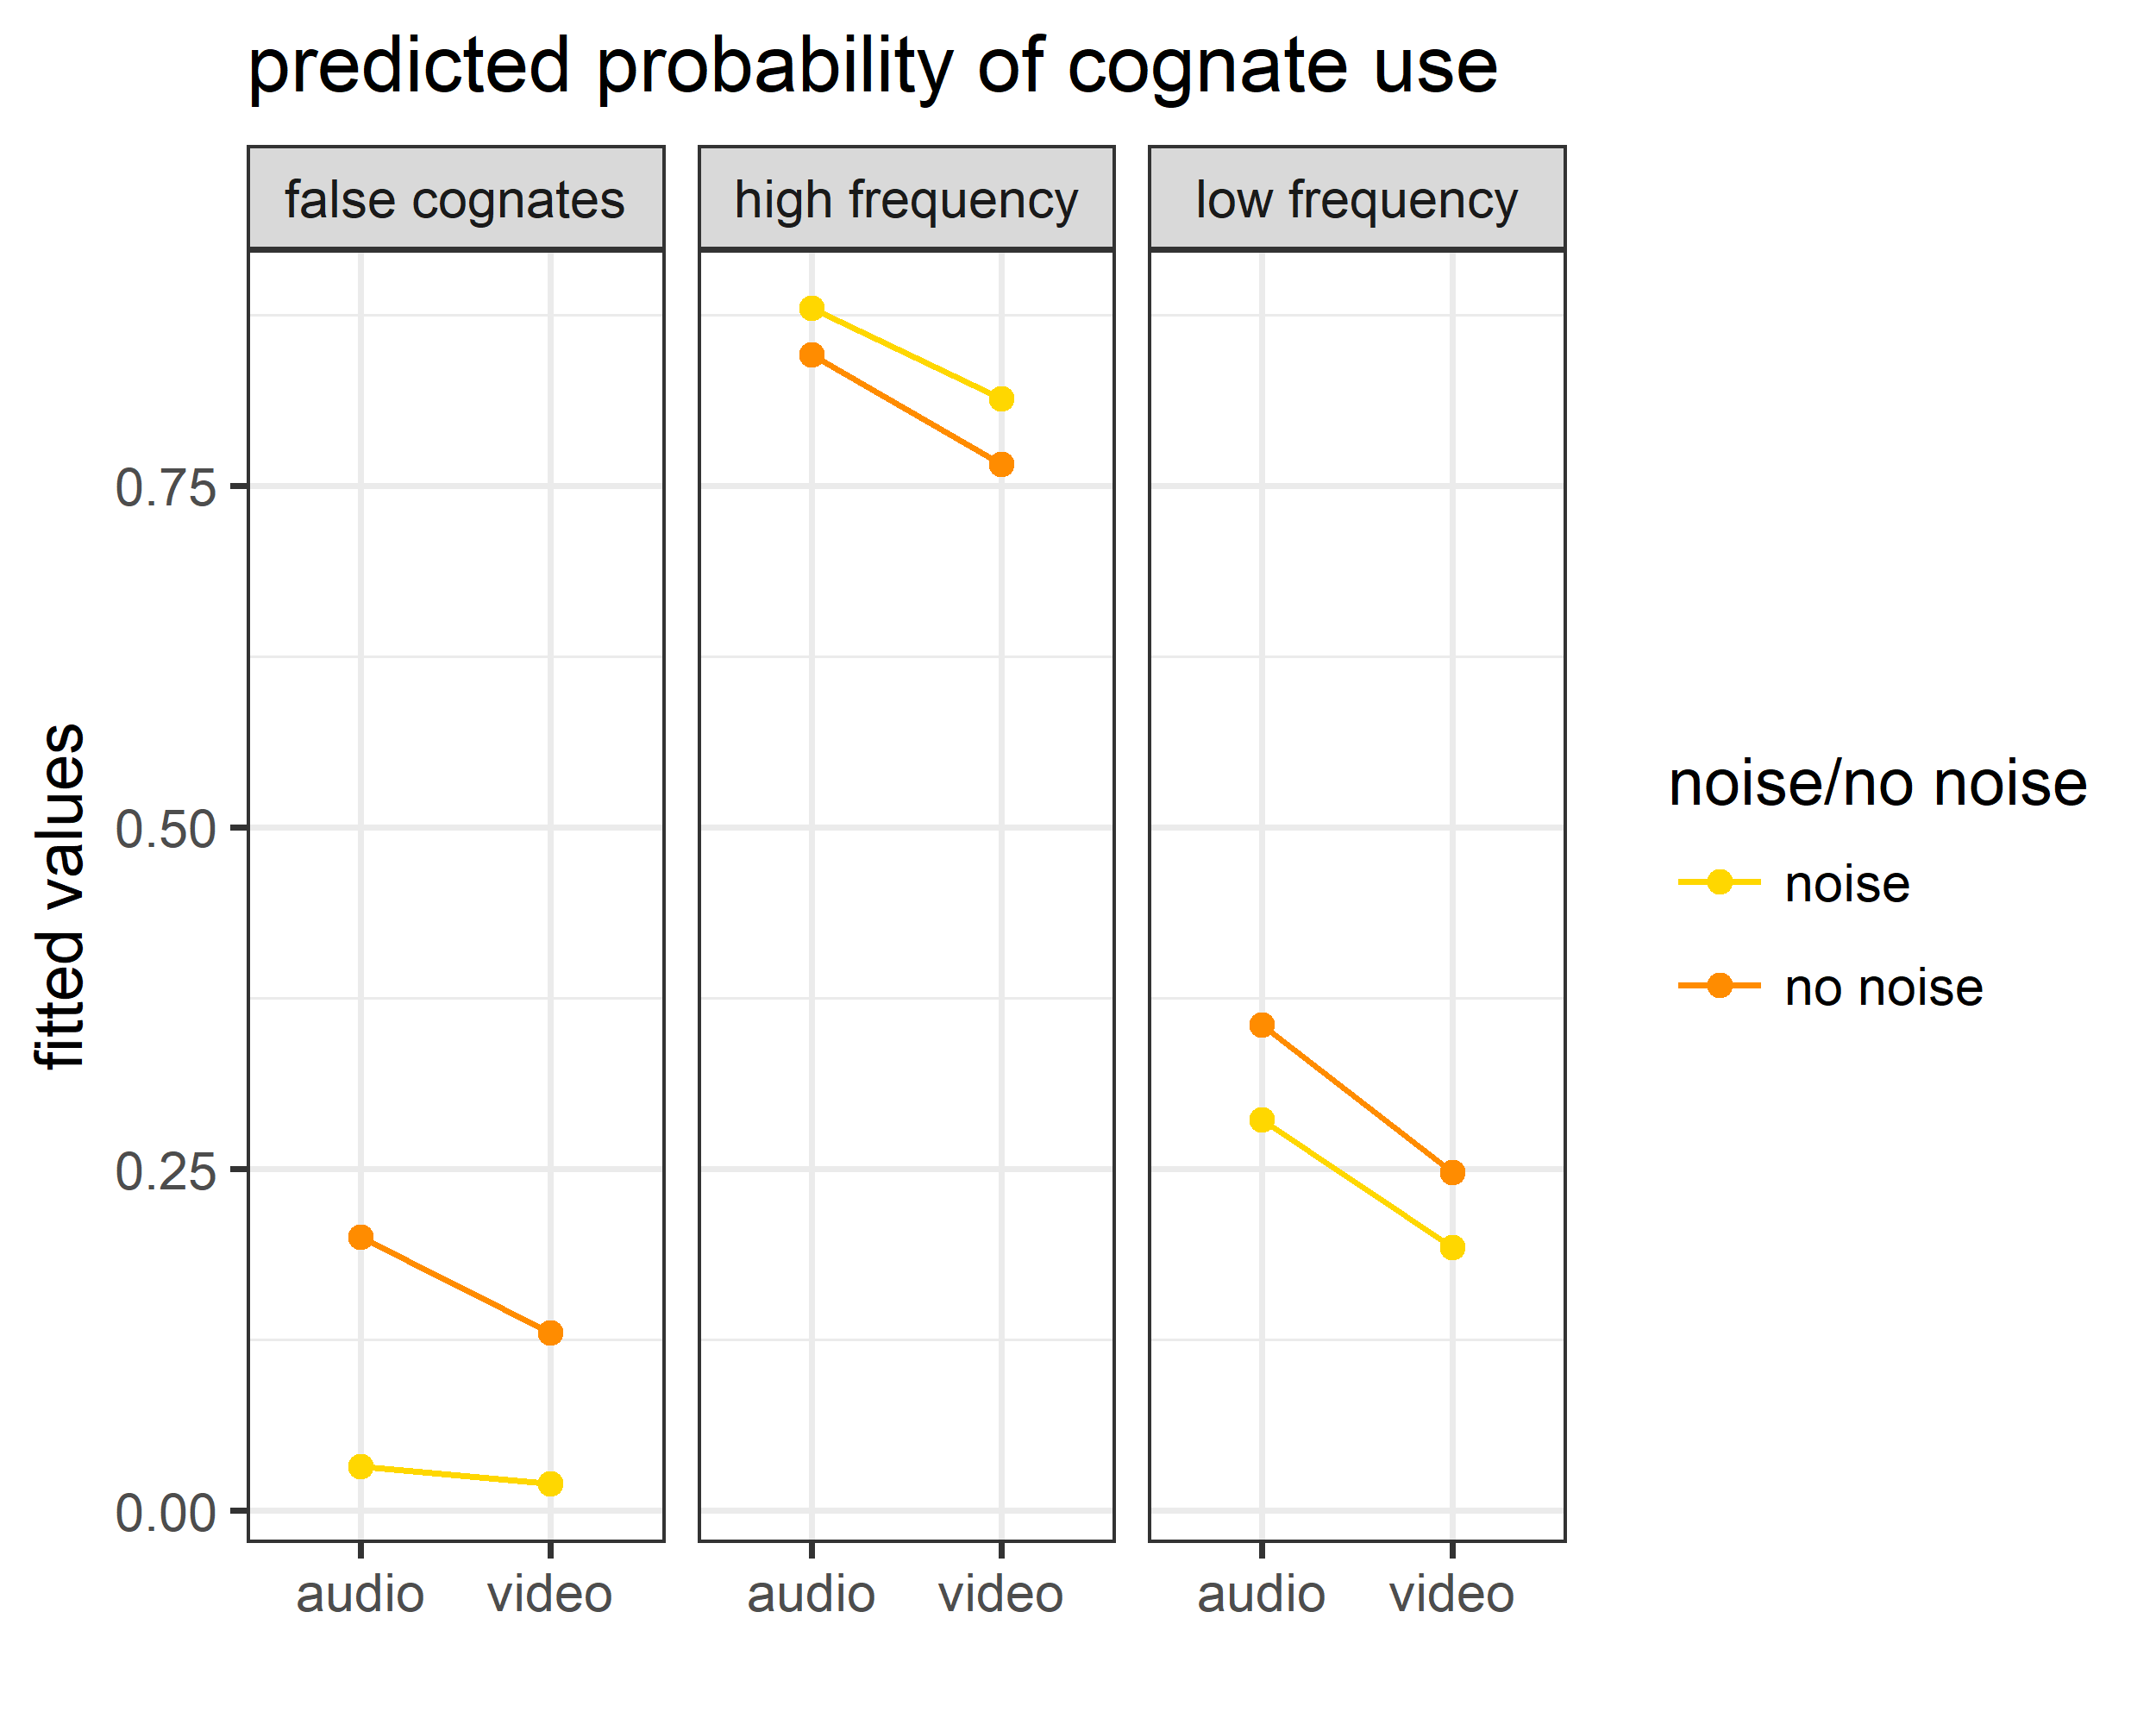
\includegraphics[height=.4\textheight]{figures/gieshoff/figure1.png}
 \caption{Estimates for cognate translation in the different conditions as predicted by the generalized linear mixed model. The estimate for the noise condition was not significant. For reasons of readability, the log odd estimates are transformed to probability estimates.}
 \label{gieshoff:fig:1}
\end{figure}

\begin{figure}[p]
 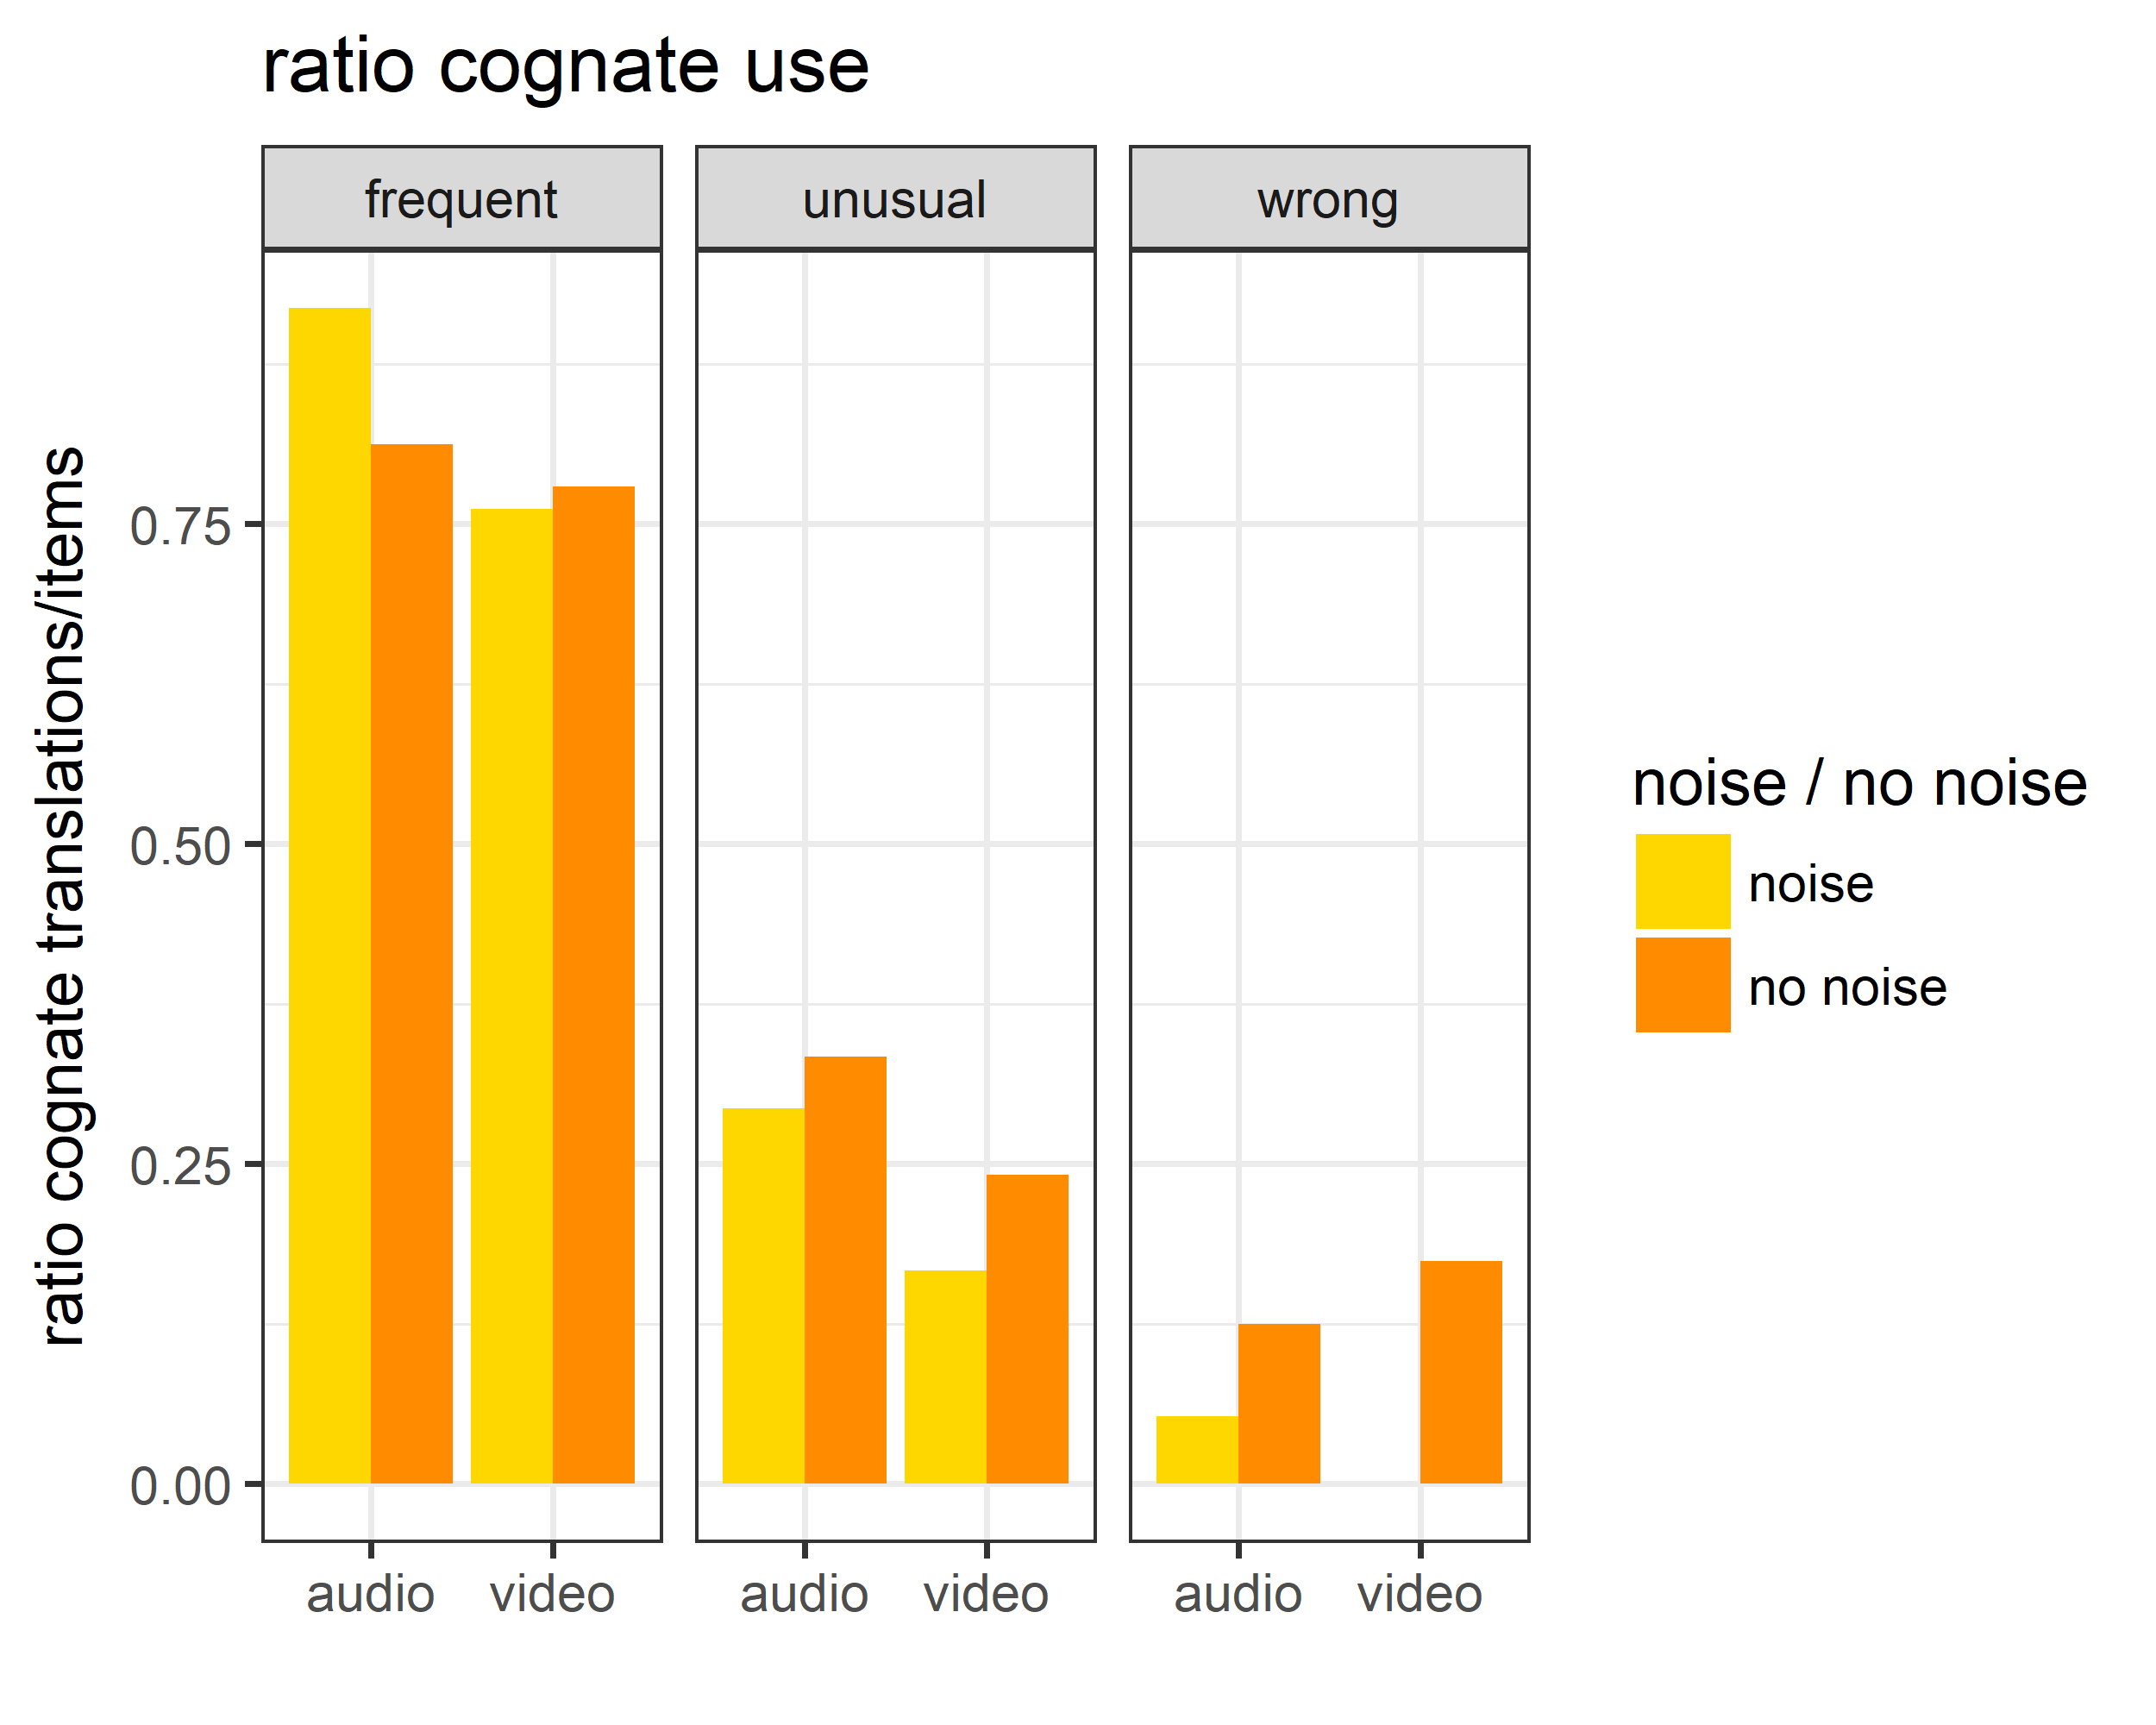
\includegraphics[height=.4\textheight]{figures/gieshoff/figure2.png}
 \caption[Observed ratio of the number realized {cognate} translations and the total number of cognates in each {cognate} category and for each condition.]{Observed ratio of the number realized {cognate} translations and the total number of cognates in each {cognate} category and for each condition.\footnotemark }
 \label{gieshoff:fig:2}
\end{figure}

Contrary to our expectation, participants did not make significantly more \isi{cognate} translations in adverse \isi{interpreting} conditions where \isi{noise} was added to the source speech than in normal \isi{interpreting} conditions. This is surprising in the sense that \isi{noise} was expected to hamper listening comprehension and therefore to drain more cognitive resources to listening comprehension which should have affected the monitoring of \isi{cognate} translations. In fact, the interaction between \isi{cognate} category and addition of background \isi{noise} estimated by the statistical model indicates that background \isi{noise} had the opposite effect for high frequency cognates on one hand and false friends on the other hand (see \figref{gieshoff:fig:1}), as can also be seen in the observed data (\figref{gieshoff:fig:2}). This paradoxical pattern is certainly due to the imbalanced distribution of \isi{cognate} translations in the three categories: the number of low frequency and false cognates was substantially lower than the number of high frequency cognates. Each text counted only five to six false friends, but 25 to 35 high frequency cognates. The probability for translating a false friend was thus much lower than for translating a high frequency \isi{cognate}. A more balanced design with an equal number of cognates in each category and a higher number of participants should help to counter this problem. \footnotetext{Plot created with ggplot \citep{Wickham2009} in R \citep{R2017}}



\section{Discussion}

The purpose of the study was to investigate the impact of \isi{audiovisual speech}, e.g. visible lip movements, and white \isi{noise} on \isi{self-monitoring} in \isi{simultaneous interpreting} by analyzing the number of \isi{cognate} translations in each condition. On the whole, participants produced very few false friends, regardless the experimental condition. This is in line with research by \citet{vanAssche2011} and by \citet{Schwartz2006} who noted that semantic information influences lexical competition and contributes to suppress lexical candidates that do not fit the semantic context.

Conforming to our hypothesis, participants translated more English cognates as \ili{German} cognates in the audio condition without visible lip movements than in the video condition with visible lip movements. Compared to the effect of the \isi{cognate} category (a decrease of \isi{cognate} translations by 52 \% for low frequency cognates and 64 \% for false friends), the effect of \isi{audiovisual speech} (a decrease by 8 \% for visible lip movements) seems rather small. Nevertheless, the effect is reliable and is not covered by the larger effect of the \isi{cognate} category which underlines the importance of \isi{audiovisual speech}. Participants seemed to be less able to detect and to inhibit \isi{cognate} translations when they interpreted the source text without seeing the lip movements of the speaker. 

One possible explanation is that visible lip movements facilitate listening comprehension in \isi{simultaneous interpreting} and allows freeing resources for \isi{self-monitoring}. Researchers observed that listening comprehension benefits from lip movements, especially in adverse listening conditions (\isi{cognitive load}, background \isi{noise}, hearing impairment, \citealt{Mattys2011, Kriegstein2008, Brancazio2006, Bernstein2004, Massaro2004}). To account for this observation, Massaro developed a Fuzzy Logical Model of Perception 1999. He assumes that neither auditory speech nor visual speech inputs are unambiguous, or to put it in other words: no signal, whether it comes from the eye or from the ear, is perfect. According to his model, a fuzzy value expresses the extent to which the new sensory information (auditory, visual, haptic or else) corresponds to a certain \textit{prototype}. A prototype describes the features of a perceptual unit of language. Auditory features for language could for example include voicing or formant information; visual features could describe the articulatory movements you see when someone pronounces a sound. The value 1, for instance, corresponds to a complete match, while the value 0 corresponds to a complete mismatch. For example, if the auditory information is ambiguous and corresponds with a value of 0.6 to prototype A and with a value of 0.5 to prototype B, but the \isi{visual input} is clearly assignable to prototype A (match of value 1), the decision is taken in favor of the prototype A and against prototype B. In this example, the \isi{visual input} provided complementary information and contributed to disambiguate the auditory input \citep{Massaro1999}.

If the auditory and \isi{visual input} provided complement each other and thereby provide a clearer signal, speech \isi{perception} processes may need fewer cognitive resources and leave more resources for other processes in \isi{simultaneous interpreting}. In his effort model for \isi{simultaneous interpreting}, \citet{Gile2009} describes four efforts which, summed up, indicate the overall resource requirements during \isi{simultaneous interpreting}: listening and comprehension, \isi{speech production}, memory and coordination. He presents several examples that illustrate how increased demands of one effort affect the other ones. For instance, a foreign accent or bad pronunciation constrains the interpreter to allocate more resources on the listening and comprehension effort. As a consequence, \isi{speech production} suffers (clumsy formulations, errors) or memory gets overloaded (information loss, \citealt[173]{Gile2009}. A similar account could hold for \isi{cognate} monitoring. Detecting inappropriate cognates needs cognitive resources. If the signal is ``noisy'' or blurred, the interpreter might devote too much of his resources to the listening and comprehension processes, which leaves insufficient resources for \isi{speech production} and monitoring. Inversely, if the signal is clearer or less ambiguous, as it is the case \isi{audiovisual speech}, interpreters may need fewer resources for listening and comprehension and can \isi{monitor} more closely their output in order to detect and inhibit uncommon \isi{cognate} translations or false friends. 

In addition to its implications for \isi{audiovisual speech} in \isi{simultaneous interpreting}, the findings reported in this paper, even though preliminary due to the low number of participants, have also methodological implications. Previous translational studies using a global evaluation of the \isi{interpreting} performance, like the informational content of the interpretation or other aspects of interpretation quality, failed to demonstrate a benefit for \isi{audiovisual speech} or \isi{visual input} in SI. The present study proposes a new method that succeeded in demonstrating a benefit for \isi{audiovisual speech} in SI. If these results can be confirmed with a larger sample, the \isi{cognate} translations analysis could prove itself a suitable method to analyze the influence of other types of \isi{visual input} or even more global problem triggers in SI, such as high source speech delivery, foreign accent, and concurrent use of other media. 

An important limitation of the study concerns the assumptions underlying our hypotheses. For instance, I assumed that interpreters can better \isi{monitor} low frequency or false \isi{cognate} translations in \isi{audiovisual speech} because they benefit from visible lip movements and have more resources available for monitoring in the video condition. However, the experimental set-up does not allow distinguishing between \isi{self-monitoring} and other processes that could explain a decrease of \isi{cognate} translations, like for example a larger activation of the semantic networks or a deeper understanding of the source text. In this respect, our study hints towards a benefit from lip movements in \isi{simultaneous interpreting} but is non-conclusive when it comes to the nature of this effect.

Furthermore, I would like to stress that the study reported in this paper was a pilot study and that the participants were student interpreters. During the years of their professional activity, interpreters acquire a certain expertise that may have an influence on how they process \isi{visual input}. For instance, their knowledge of their working languages and the ability to discriminate the sounds of these languages improves over the years. Consequently, the benefit of visible lip movements could diminish. Further research is necessary to extend the findings to professional interpreters and to confirm them with a larger sample. 

To summarize, the results showed an increase of \isi{cognate} translations when the interpreters worked without visible lip movements. One explanation might be that \isi{self-monitoring} is less effective in this condition because conference interpreters need to allocate more of their resources to the comprehension of the source text. The findings of this study point out the importance of \isi{visual input} in \isi{simultaneous interpreting} and its integration in models of \isi{simultaneous interpreting}.

\section*{Acknowledgments}

I am very grateful to Joachim Kildau and Katharina Oster for their helpful comments on earlier drafts of this paper.

\sloppy
\printbibliography[heading=subbibliography,notkeyword=this]
\end{document}

% \begin{styleLiteraturverzeichnis}
% @book{AIIC2016,
% 	address = {Retrieved 03 28, 2016, from aiic},
% 	author = {AIIC, W.},
% 	note = {//aiic.net/page/151/hiring-si-equipment-tips-for-conference-organisers/lang/1},
% 	publisher = {http:},
% 	title = {\textit{Hiring SI equipments - tips for conference organisers}},
% 	year = {2016}
% }
% \end{styleLiteraturverzeichnis}
% 
% \begin{styleBibliography}
% @misc{\citet{Audacity2015,
% 	author = {\citet{Audacity},
% 	title = {}. \textit{Audacity}. },
% 	url = {http://audacityteam.org/copyright},
% 	year = {2015}
% }
% \end{styleBibliography}
% 
% 
% \begin{styleBibliography}
% Acheson, D., Ganushchak, L., Christoffels, I., \& Hagoort, P. (2012). Conflict monitoring in \isi{speech production}: Physiological evidence from bilingual picture naming. \textit{Brain \& Language, 123}, pp. 131-136.
% \end{styleBibliography}
% 
% \begin{styleBibliography}
% @article{Anderson1994,
% 	author = {Anderson, L},
% 	note = {. Amsterdam, Philadelphia: John Benjamins.},
% 	pages = {101-120},
% 	title = {Simultaneous Interpretation: Contextual and Translation Aspects. In S. Lambert, \& B. Moser-Mercer, \textit{Bridging the Gap. Empirical Research in Simultaneous Interpretation} (vol},
% 	volume = {3},
% 	year = {1994}
% }
% \end{styleBibliography}
% 
% 
% \begin{styleBibliography}
% Barr, D., Levy, R. S., \& Tily, H. (2013). Random effects structure for confirmatory hypothesis testing: Keep it maximal. \textit{Journal of Memory and Language, 68}(3), pp. 255-278.
% \end{styleBibliography}
% 
% \begin{styleBibliography}
% Bates, D., Maechler, M., Bolker, B., \& Walker, S. (2015). Fitting Linear Mixed-Effects Models Using lme4. \textit{Journal of Statistical Software, 67}(1), pp. 1-48.
% \end{styleBibliography}
% 
% 
% \begin{styleLiteraturverzeichnis}
% Bernstein, L., Auer, E., \& Takayanagi, S. (2004). Auditory speech detection in \isi{noise} enhanced by li-reading. \textit{Speech Communication, 44}, S. 5-18.
% \end{styleLiteraturverzeichnis}
% 
% \begin{styleLiteraturverzeichnis}
% Brancazio, L., Best, C., \& Fowler, C. (2006). Visual Influences on Perception of Speech and Non-Speech Vocal Tract Events. \textit{Language and Speech, 49}(1), S. 21-53.
% \end{styleLiteraturverzeichnis}
% 
% \begin{styleBibliography}
% Calvert, G., \& These, T. (2004). Multisensory integration: Methodological approaches and emerging principles in the human brain. \textit{Journal of Physiology-Paris, 98}, pp. 191-205.
% \end{styleBibliography}
% 
% 
% \begin{styleBibliography}
% Christoffels, I., de Groot, A., \& Walorp, L. (2003). Basic skills in a complex task: A graphical model relating memory a lexical retrieval to \isi{simultaneous interpreting}. \textit{Bilingualism: Language and Cognition, 6}, pp. 201-2011.
% \end{styleBibliography}
% 
% \begin{styleBibliography}
% Christoffels, I., Firk, C., \& Schiller, N. (2007). Bilingual language control: A event-related brain potential study. \textit{Brain Research, 1147}, pp. 192-208.
% \end{styleBibliography}
% 
% \begin{styleBibliography}
% Costa, A., Santesteban, M., \& Cano, A. (2005). On the facilitory effect of \isi{cognate} words in bilingual \isi{speech production}. \textit{Brain and Language, 94}, pp. 94-103.
% \end{styleBibliography}
% 
% %\begin{styleBibliography}
% Costa, A., Colomé, A., Gómez, O. and Sebastián-Gallés, N. (2003). Another look at crosslanguage competition in bilingual \isi{speech production}: Lexical and phonological factors. Bilingualism: Language and Cognition, 6, pp 167-179 doi:10.1017/S1366728903001111
% \end{styleBibliography}
%
%
%
% \begin{styleBibliography}
% @misc{Davies2009,
% 	author = {Davies, M},
% 	title = {\textit{Word frequency data. Corpus of Contemporary American English}. (Brigham Young University) Retrieved 03/15/2014, from },
% 	url = {http://www.wordfrequency.info/},
% 	year = {2009}
% }
% \end{styleBibliography}
% 
% \begin{styleBibliography}
% de Groot, A., \& Nas, G. (1991). Lexical Representation of Cognates and Noncognates in Compound Bilinguals. \textit{Journal of Memory and Language, 30}, pp. 90-123.
% \end{styleBibliography}
% 
% \begin{styleBibliography}
% @book{De2005,
% 	address = {La traduction à vue en interprétation simultanée: quelle opérationnalité ambitionner? \textit{Meta},
% 	author = {De Laet, F.,  and  Plas, R. V.},
% 	publisher = {journal des traducteurs, 50}(4), no page indicated},
% 	year = {2005}
% }
% \end{styleBibliography}
% 
% \begin{styleBibliography}
% Dijkstra, T., Grainger, J., \& van Heuven, W. (1999). Recognition of Cognates and Interlingual Homographs: the Neglected Role of Phonology. \textit{Journal of Memory and Language, 41}, pp. 469-518.
% \end{styleBibliography}
% 
% \begin{styleBibliography}
% Dijkstra, T., Miwa, K., Brummelhuis, B., Sappelli, M., \& Baayen, H. (2010). How cross-language similiarity an task demands affect \isi{cognate} recognition. \textit{Journal of Memory and Language, 62}, pp. 284-301.
% \end{styleBibliography}
% 
% \begin{styleBibliography}
% Dijkstra, T., van Hell, J., \& Brenders, P. (2015). Sentence context effects in bilingual word recognition: Cognate status, sentence language, and semantic constraint. \textit{Bilingualism: Language and Cognition, 18}, pp. 597-613.
% \end{styleBibliography}
% 
% \begin{styleBibliography}
% Dijkstra, T., van Jaarsveld, H., \& ten Brinke, S. (1998). Interlingual homograph recognition: Effects of task demands and language intermixing. \textit{Bilingualism: Language and Cognition, 1}, pp. 55-61.
% \end{styleBibliography}
% 
% \begin{styleBibliography}
% Dong, Y., \& Lin, J. (2013). Parallel processing of the \isi{target language} during \isi{source language} comprehension in \isi{interpreting}. \textit{Bilingualism: Language and Cognition, 16}, pp. 682-692.
% \end{styleBibliography}
% 
% 
% \begin{styleBibliography}
% Gerver, David. 1975. “A psychological approach to \isi{simultaneous interpreting}”. Meta 20 (2): 119-128
% \end{styleBibliography}
%
%
% \begin{styleBibliography}
% @book{Gile2009,
% 	address = {\textit{Basic Concepts ad Models for Interpreter and Translator Training.} Amsterdam/Philadelphia},
% 	author = {Gile, D.},
% 	publisher = {John Benjamins},
% 	year = {2009}
% }
% \end{styleBibliography}
% 
% \begin{styleBibliography}
% Giraud, A. L., \& Truy, E. (2002). The contribution of visual areas to speech comprehension. a PET study in cochelar implants patients and normal-hearing subjects. \textit{Neuropsychologia, 40}, pp. 1562-1569.
% \end{styleBibliography}
% 
% 
% \begin{styleBibliography}
% @book{Hermetsberger2002,
% 	address = {English-\ili{German} Dictionary},
% 	editor = {Hermetsberger, P.},
% 	note = {//www.dict.cc/},
% 	publisher = {http:},
% 	title = {\textit{dict.cc. Deutsch-Englisch Wörterbuch}. (dict.cc GmbH) Retrieved 12/10/2014, from dict.cc},
% 	year = {2002}
% }
% \end{styleBibliography}
% 
% 
% \begin{styleLiteraturverzeichnis}
% International Organization for Standardization. (2603:1998). Booths for simultaneous interpretation. General characteristics and equipment. 13. Vernier, Geneva, Switzerland.
% \end{styleLiteraturverzeichnis}
% 
% \begin{styleBibliography}
% Jared, D., \& Kroll, J. (2001). Do Bilinguals Activate Phonological Representations in One or Both of Their Languages When Naming Words? \textit{Journal of Memory and Language, 44}, pp. 2-31.
% \end{styleBibliography}
% 
% \begin{styleBibliography}
% Kessel, R; Gecht, J.; Forkmann, T.; Drueke, B.; Guaggel, S; Mainz, V. (2014). Metacognitive monitoring of attention performance and its influencing factors. \textit{Psychological Research. 78}, pp. 597-607.
% \end{styleBibliography}
% 
% \begin{styleBibliography}
% Kriegstein, K. (2008). Simulation of talking faces in the human brain improves auditory speech recognition. \textit{Proceedings of the National Academy of Sciences of the United States of America, 105}(18), pp. 6747-6752.
% \end{styleBibliography}
% 
% \begin{styleBibliography}
% Lambert, S. (2004). Shared Attention during Sight Translation, Sight Interpretation and Simultaneous Interpretation. \textit{Meta: journal des traducteurs, 49}(2), pp. 294-306.
% \end{styleBibliography}
% 
% 
% \begin{styleBibliography}
% Lewandowski, L., \& Kobus, D. (1993). The Effects of Redundancy of Bimodal Word Processing. \textit{Human Performance, 6}(3), pp. 229-239.
% \end{styleBibliography}
% 
% \begin{styleBibliography}
% @book{Linguee2015,
% 	address = {English-\ili{German} dictionary},
% 	author = {Linguee GmbH},
% 	note = {//www.linguee.de/},
% 	publisher = {http:},
% 	title = {\textit{Linguee. Deutsch-Englisch Wörterbuch}. Retrieved 12/10/2014 from Linguee},
% 	year = {2015}
% }
% \end{styleBibliography}
% 
% \begin{styleLiteraturverzeichnis}
% Massaro, D., \& Light, J. (2004). Using Visible Speech to Train Perception and Production of Individuals with Hearing Loss. \textit{Journal of Speech, Language and Hearing Research, 47}(2), pp. 304-320.
% \end{styleLiteraturverzeichnis}
% 
%\begin{styleBibliography}
% Massaro, D., & Cohen, M. (1999). Speech \isi{perception} in perceivers with hearing loss: Synergy of multiple modalities. Journal of Speech, Language and Hearing Research, 42(1), pp. 21-41.
% \end{styleBibliography}
%
%
%
% \begin{styleBibliography}
% Mattys, S., \& Wiget, L. (2011). Effects of \isi{cognitive load} on speech recognition. \textit{Journal of Memory and Language, 65}, pp. 145-160.
% \end{styleBibliography}
% 
% \begin{styleBibliography}
% Mc Gurk, H., \& MacDonald, J. (1976). Hearing lips and seeing voices. \textit{Nature, 264}, pp. 746-748.
% \end{styleBibliography}
% 
% \begin{styleBibliography}
% McGettigan, C. (2012). Speech Comprehension aided by Multiple Modalities: Behavioral and Neural Interactions. \textit{Neuropsychologia, 50}, pp. 762-776.
% \end{styleBibliography}
% 
% \begin{styleBibliography}
% Moser-Mercer, B. (2005). Meta: journal des traducteurs. \textit{Remote-Interpreting: Issues of Multi-Sensory Intergratino in a Multilingual Task, 50}(2), S. 727-738.
% \end{styleBibliography}
% 
% 
% \begin{styleLiteraturverzeichnis}
% Oomen, C., \& Postma, A. (2001). Effects of divided attention on filled \isi{pauses} and repetitions. \textit{Journal of Speech, Language and Hearing Research, 44}(5), pp. 997-1004.
% \end{styleLiteraturverzeichnis}
% 
% 
% \begin{styleBibliography}
% @book{Paradis2004,
% 	address = {\textit{A Neurolinguistic Theory of Bilingualism.} Amsterdam, Philadelphia},
% 	author = {Paradis, M.},
% 	publisher = {John Benjamins},
% 	year = {2004}
% }
% \end{styleBibliography}
% 
% \begin{styleBibliography}
% Peeters, D., Dijkstra, T., \& Grainger, J. (2013). The representation of identical cognates by late \isi{bilinguals}: RT ad ERP effects. \textit{Journal of Memory and Language, 68}, pp. 315-332.
% \end{styleBibliography}
% 
% \begin{styleLiteraturverzeichnis}
% Postma, A. (2000). Detection of errors during \isi{speech production}: a review of speech monitoring models. \textit{Cognition, 77}, pp. 97-131.
% \end{styleLiteraturverzeichnis}
% 
% \begin{styleBibliography}
% @misc{Quasthoff2013,
% 	author = {Quasthoff, U., Goldhahn, D.,  and  Heyer, G},
% 	title = {/02). \textit{Technical Report Series on Corpus Building. Deutscher \citealt{Wortschatz2012}}. (Universität Leipzig. Abteilung Automatische Sprachverarbeitung) Retrieved from },
% 	url = {http://corpora.informatik.uni-leipzig.de/index.php?corpusId=nld\_web\_2002},
% 	year = {2013}
% }
% \end{styleBibliography}
% 
% \begin{styleBibliography}
% @misc{R2014,
% 	author = {R Core \citet{Team},
% 	title = {}. \textit{A language and environment for statistical computing.} Retrieved from },
% 	url = {http://R-project.org/},
% 	year = {2014}
% }
% \end{styleBibliography}
% 
% \begin{styleBibliography}
% Rennert, S. (2008). Visual Input in Simultaneous Interpreting. \textit{Meta: journal des traducteurs, 53}(1), pp. 204-217.
% \end{styleBibliography}
% 
% 
% \begin{styleBibliography}
% Rosenblum, L. (2008). Speech \isi{perception} as a multimodal phenomenon. \textit{Current Directions in Psychological Science, 17}(6), pp. 405-409.
% \end{styleBibliography}
% 
% \begin{styleBibliography}
% Schwartz, A., \& Kroll, J. (2006). Bilingual lexical activiation in sentence context. \textit{Journal of Memory and Language, 55}, pp. 197-212.
% \end{styleBibliography}
% 
% \begin{styleBibliography}
% Seeber, K., & Kerzel, D. (2012). Cognitive Load in Simultaneous Interpreting - Model meets data. International Journal of Bilingualism, 16(2), pp. 228-242.
% \end{styleBibliography}
%
% \begin{styleBibliography}
% @book{Setton1999,
% 	address = {\textit{Simultaneous Interpretation - A cognitive-pragmatic analysis.} Amsterdam/Philadelphia},
% 	author = {Setton, R.},
% 	publisher = {John Benjamin's},
% 	year = {1999}
% }
% \end{styleBibliography}
% 
% \begin{styleBibliography}
% Shook, A. (2013). The Bilingual Language Interaction Network for Comprehension of Speech. \textit{Bilingualism: Language and Cognition, 16}(2), pp. 304-324.
% \end{styleBibliography}
% 
% \begin{styleBibliography}
% Starreveld, P., de Groot, A., Rossmark, B., \& van Hell, J. (2015). Parallel language activation during word processing in \isi{bilinguals}: Evidence from word production in sentence context. \textit{Bilingualism: Language and Cognition}, pp. 1-19.
% \end{styleBibliography}
% 
% 
% \begin{styleBibliography}
% van Assche, E., Drieghe, D., Duyck, W., Welvaert, M., \& Hartsuiker, R. (2011). The influence of semantic constraints on bilingual word recognition during sentence reading. \textit{Journal of Memory and Language, 64}, pp. 88-107.
% \end{styleBibliography}
% 
% \begin{styleBibliography}
% van Assche, E., Duyck, W., Hartsuiker, R., \& Diependaele, K. (2009). Does Bilingualism Change Native-Language-Reading? \textit{Psychological Science, 20}(8), pp. 923-927.
% \end{styleBibliography}
% 
% \begin{styleBibliography}
% van Hell, J., \& de Groot, A. (1998). Conceptual representation in bilingual memory: Effects of concreteness and \isi{cognate} status in word association. \textit{Bilingualism: Language and Cognition, 1}, pp. 193-211.
% \end{styleBibliography}
% 
% 
% \begin{styleBibliography}
% @book{Wickham2009,
% 	address = {\textit{ggplot2: elegant graphics for data analysis.} New York},
% 	author = {Wickham, H.},
% 	publisher = {Springer},
% 	year = {2009}
% }
% \end{styleBibliography}
